\section{Executing fuzzed data}

\begin{figure}[h!]
    \centering
    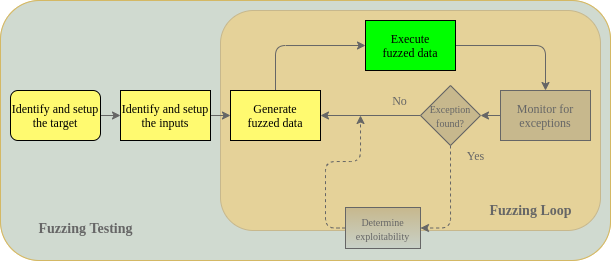
\includegraphics[width=\linewidth]{Chapter3/fuzzing_phase4.png}
\end{figure}

After the selection of the inputs for execution, Waffle instantiates an environment for the execution of the target program. In this environment, Waffle shares memory with the program and collects the features necessary to enhance the performance of our fuzzer.

